%=============================================================================
%   Pentomino by Pentomino
%   Reporte de pentominos - Experiment Results
%   Servicio social - Laura Natalia Borbolla Palacios
%=============================================================================

\subsection{Pentomino By Pentomino}
For each pentomino entry there will be an isometric figure to ilustrate the
initial scenario. The pentominoes are alphabetically ordered and will be included
only some moments of the evolution; ergo, the appendix contains the complete
evolution of each pentomino.

% O PENTOMINO ==================================================================
\subsubsection{O-Pentomino}
\label{sec:o-pentomino}

This is, as seen in figure~\ref{fig:iso-pent-o}, the simplest pentomino in the
set. As seen in the figure~\ref{fig:ss-pent:o-osc}, in the $9^{th}$ generation,
it splits into two identical oscillators (see figure~\ref{fig:iso-osc-1}),
sadly, each one obstructs the way of the other and by the $21^{th}$ generation,
all the cells are dead.

\begin{figure}
	\centering
	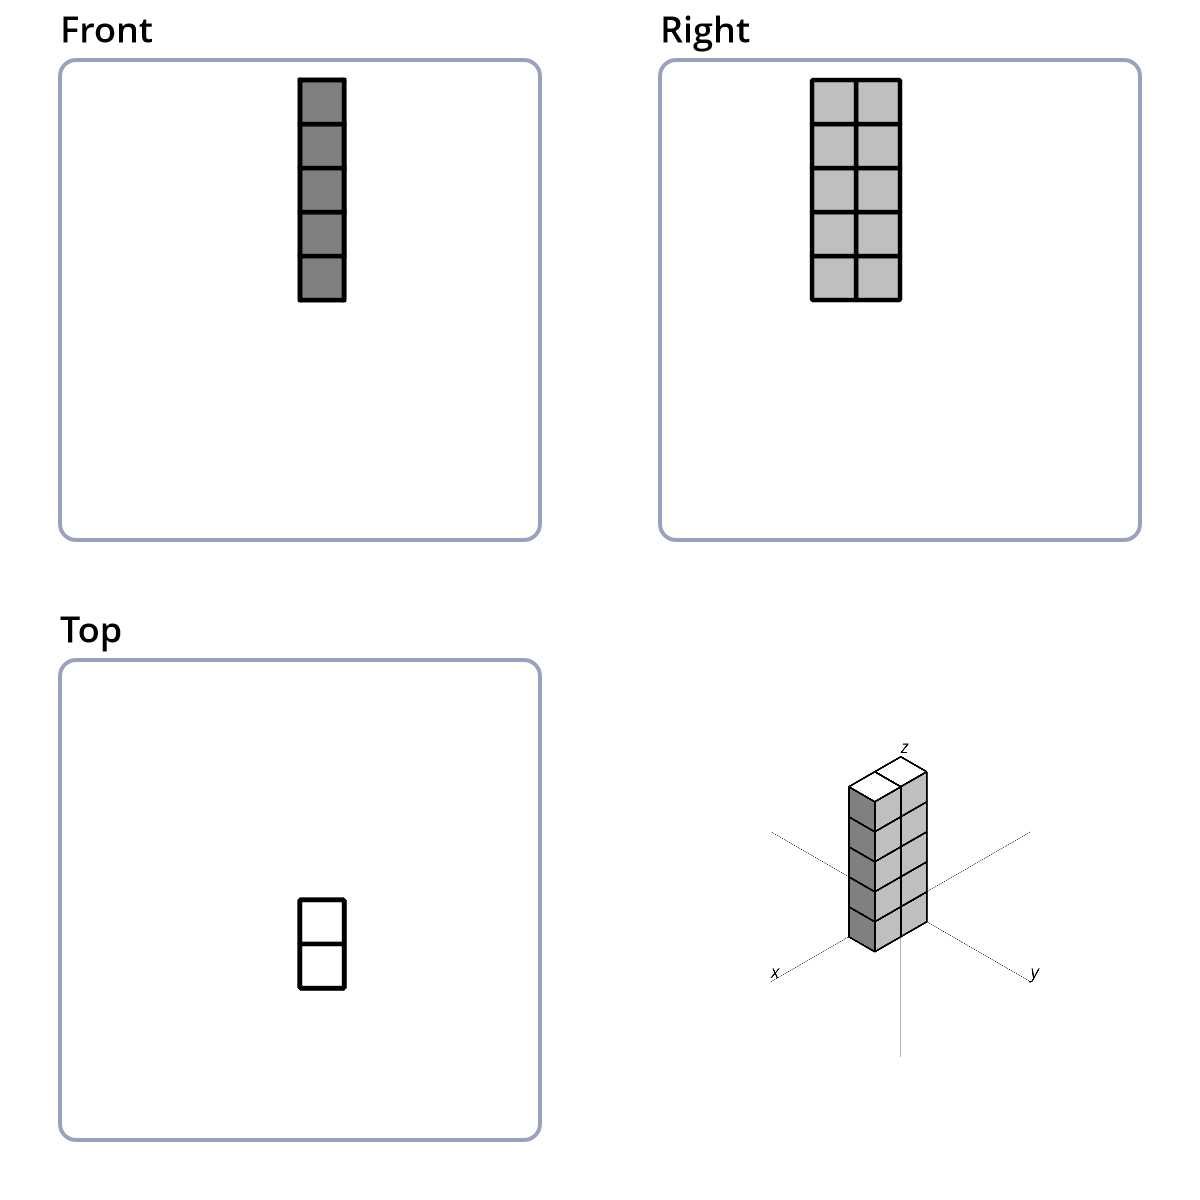
\includegraphics[scale=0.3]{iso_diagrams/o.png}
	\caption{Isometric of the O-pentomino.}
  \label{fig:iso-pent-o}
\end{figure}

\begin{figure}
	\centering
	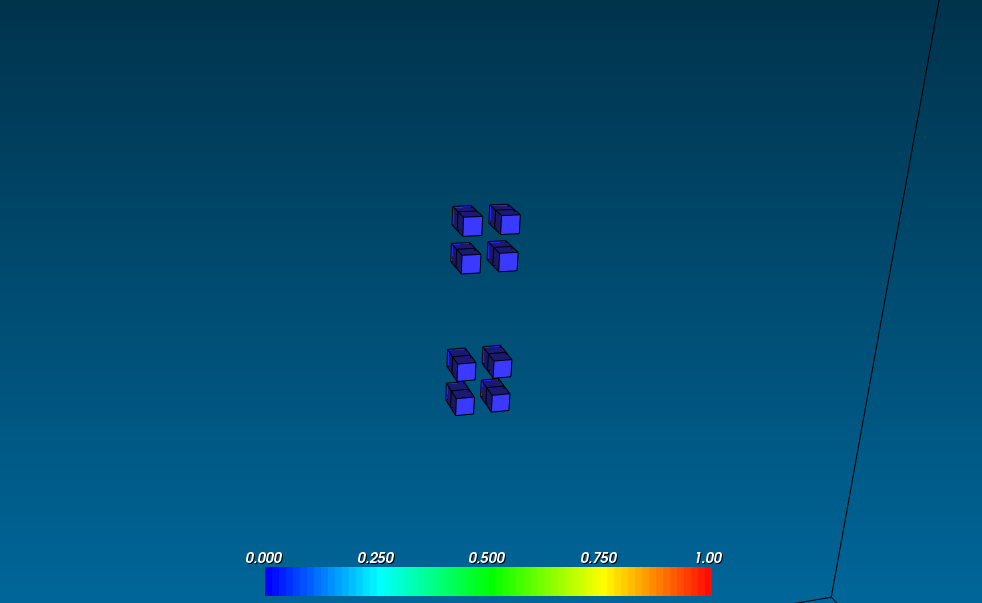
\includegraphics[scale=0.3]{pentominoes_ss/o_osc.png}
	\caption{Evolution of the O-Pentomino, $9^{th}$ generation.}
  \label{fig:ss-pent:o-osc}
\end{figure}

% P PENTOMINO ==================================================================
\subsubsection{P-Pentomino}
\label{sec:p-pentomino}

This pentomino (see figure~\ref{fig:iso-pent-p}) is quite interesting; three
configurations can bee seen whithin less than 47 generations. The first one to
appear is a puffer train (see figure~\ref{fig:iso-puffer-1}), latter, the first
(and one of the simplest) glider appears (see figure~\ref{fig:iso-glider-1});
finally, another glider appears (see figure~\ref{fig:iso-glider-2}).

Figure~\ref{fig:ss-pent:p-42} shows the state of the evolution of the
p-pentomino in the $42^{th}$ generation; the puffer can be seen in the north
of the evolution; while the gliders are located in the south of the population.

The simulation of this pentomino stopped at 210 generations because the space
was overcrowded.

\begin{figure}
	\centering
	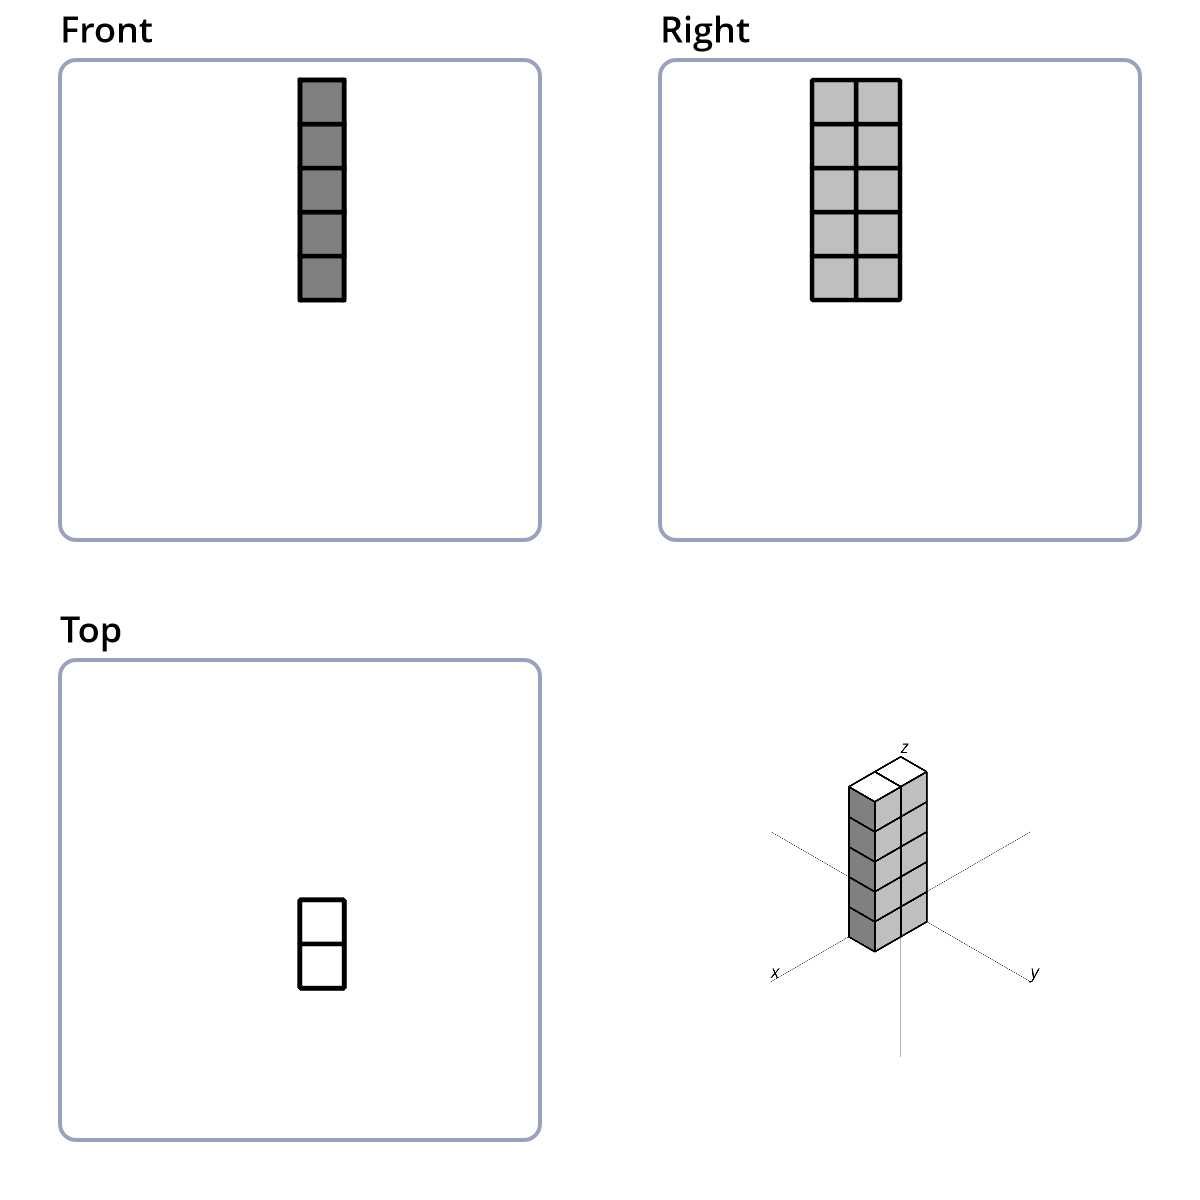
\includegraphics[scale=0.3]{iso_diagrams/o.png}
	\caption{Isometric of the P-pentomino.}
  \label{fig:iso-pent-p}
\end{figure}


\begin{figure}
	\centering
	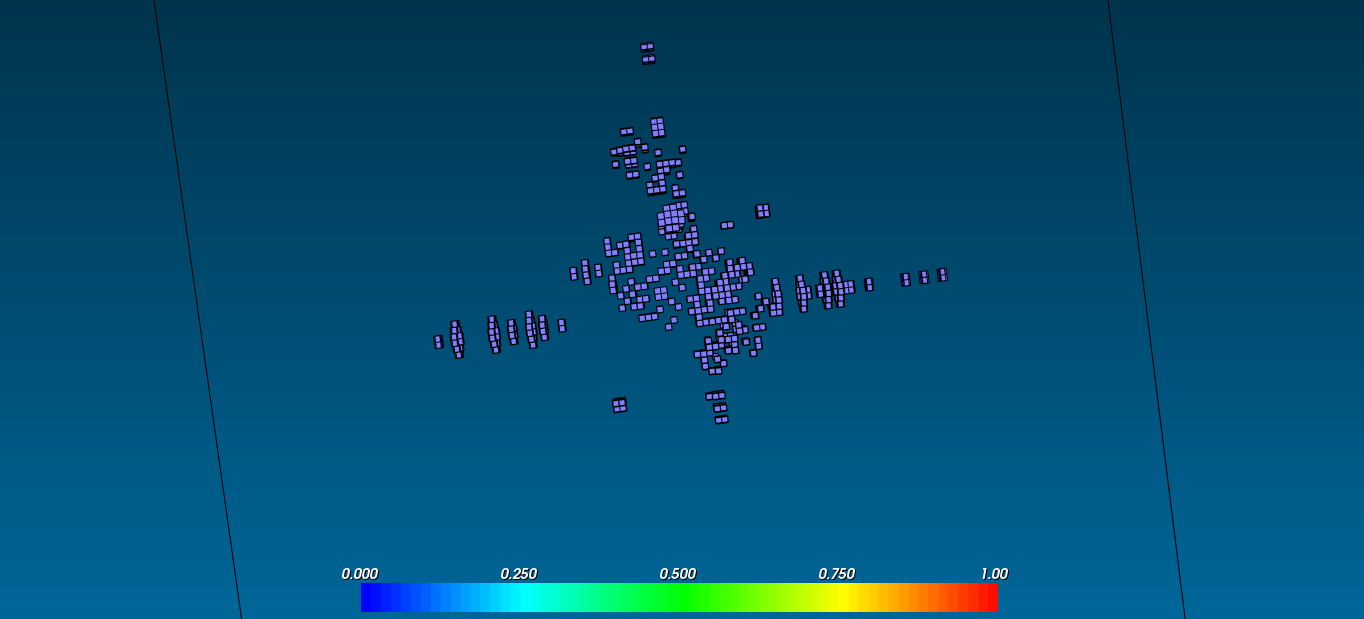
\includegraphics[scale=0.3]{pentominoes_ss/p_42.png}
	\caption{Evolution of the P-Pentomino, $42^{th}$ generation.}
  \label{fig:ss-pent:p-42}
\end{figure}

\begin{figure}
	\centering
	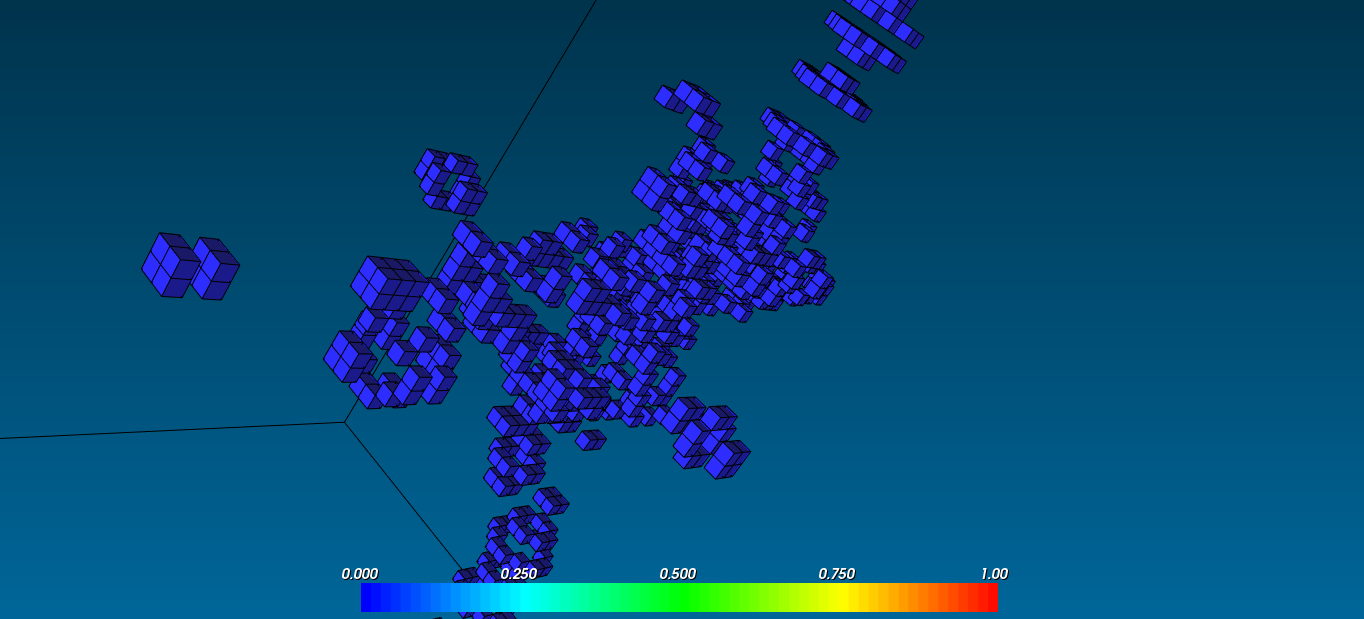
\includegraphics[scale=0.3]{pentominoes_ss/p_42_puffer.png}
	\caption{Evolution of the P-Pentomino, zoomed puffer train, $42^{th}$
	generation.}
  \label{fig:ss-pent:p-42}
\end{figure}

\begin{figure}
	\centering
	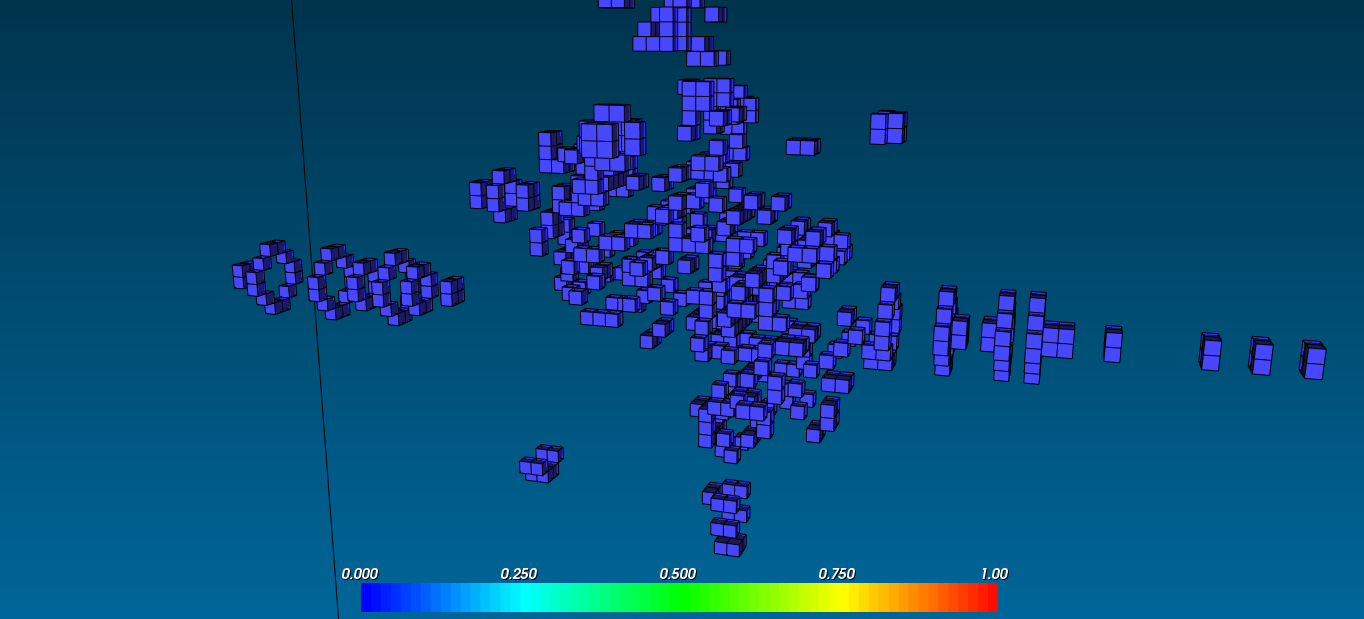
\includegraphics[scale=0.3]{pentominoes_ss/p_42_gliders.png}
	\caption{Evolution of the P-Pentomino, zoomed gliders, $42^{th}$ generation.}
  \label{fig:ss-pent:p-42}
\end{figure}


% Q PENTOMINO ==================================================================
\subsubsection{Q-Pentomino}
\label{sec:q-pentomino}
This pentomino (see figure~\ref{fig:iso-pent-q}) shows in ten generations, two
structures, one is a puffer train (see figure~\ref{fig:iso-puffer-1}), and a
\textit{modified} glider: the glider-1 (see figure~\ref{fig:iso-glider-1}) with
a satellite (see figure~\ref{fig:iso-glider-3}). The evolution of the $10^{th}$
generation with both structures can be seen in figure~\ref{fig:ss-pent:q-10}.

As shown in~\ref{fig:ss-pent:q-50}, in the $50^{th}$ generation, a mirroed
glider-4 (see figure~\ref{fig:iso-glider-4}) emerges, both in the north and
south of the population; the figures \ref{fig:ss-pent:q-50-gliders} and
\ref{fig:ss-pent:q-52-gliders} show the gliders, zoomed, in the $50^{th}$ and
$52^{th}$ generation, respectively.

The simulation of this pentomino stopped at 109 generations because the space
was overcrowded.

\begin{figure}
	\centering
	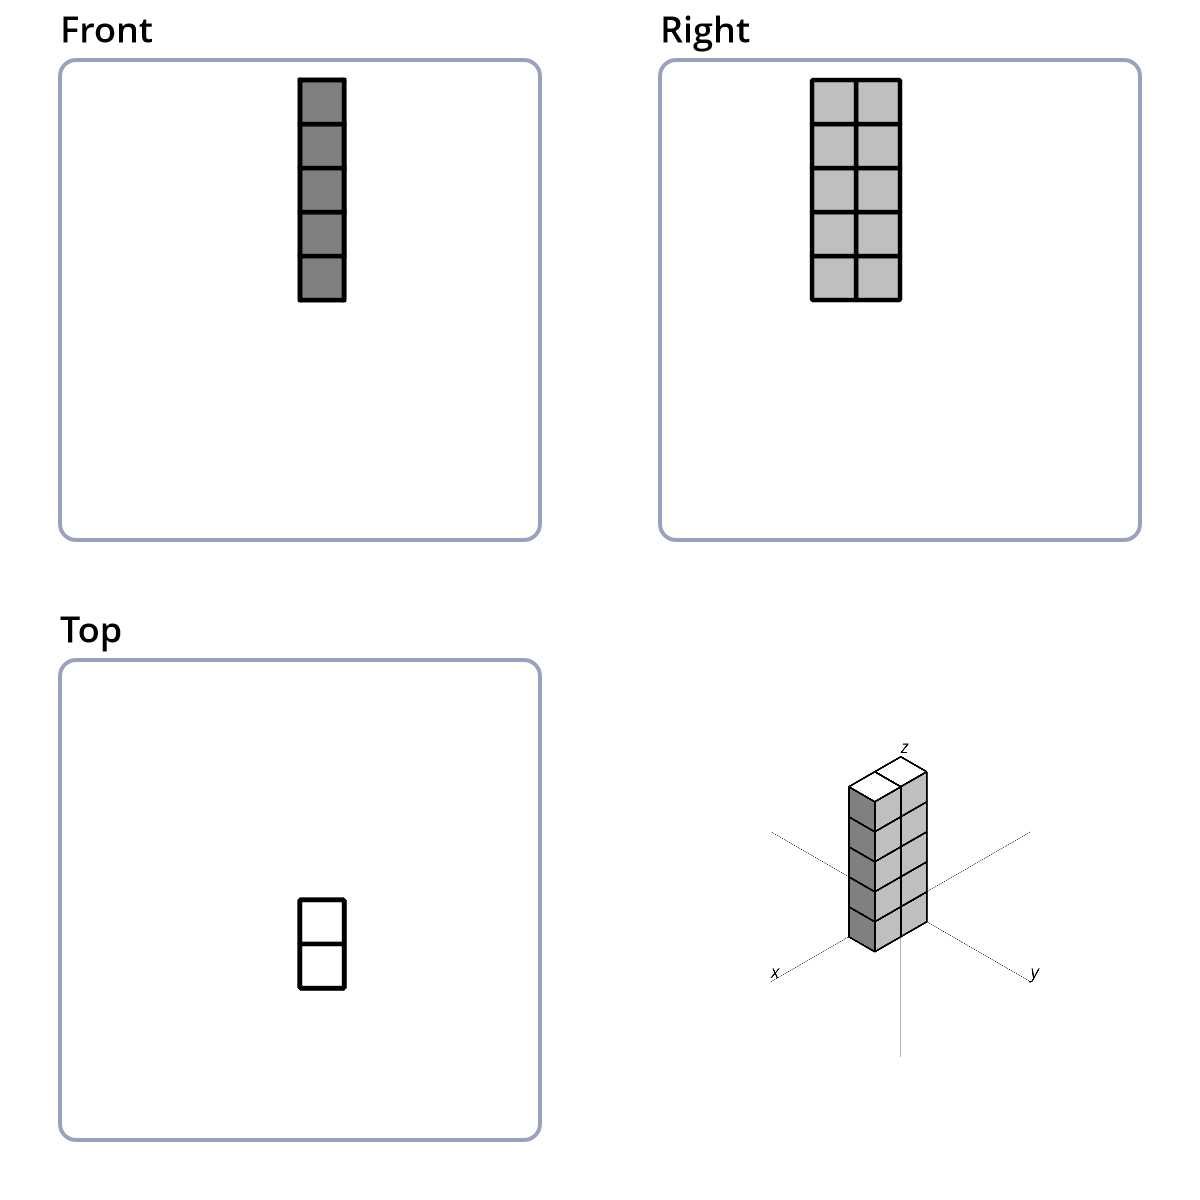
\includegraphics[scale=0.3]{iso_diagrams/o.png}
	\caption{Isometric of the Q-pentomino.}
  \label{fig:iso-pent-q}
\end{figure}

\begin{figure}
	\centering
	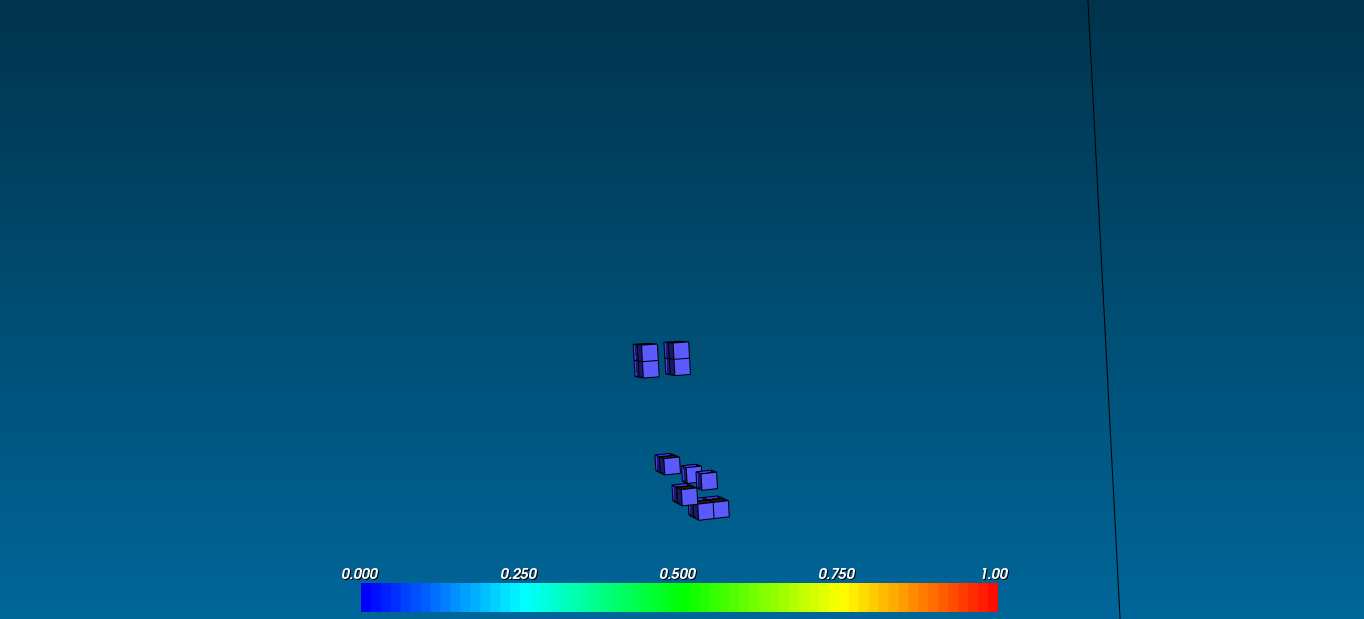
\includegraphics[scale=0.3]{pentominoes_ss/q_10.png}
	\caption{Evolution of the Q-Pentomino, $10^{th}$ generation.}
  \label{fig:ss-pent:q-10}
\end{figure}

\begin{figure}
	\centering
	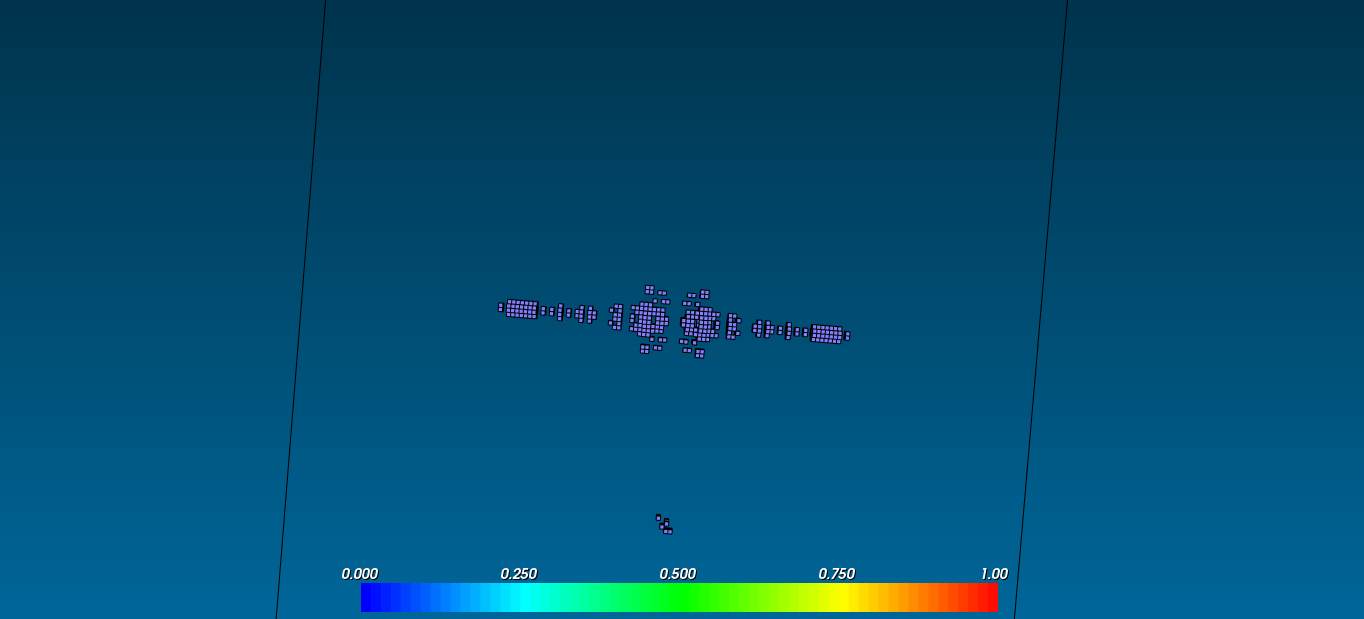
\includegraphics[scale=0.3]{pentominoes_ss/q_50.png}
	\caption{Evolution of the Q-Pentomino, $50^{th}$ generation.}
  \label{fig:ss-pent:q-50}
\end{figure}

\begin{figure}
	\centering
	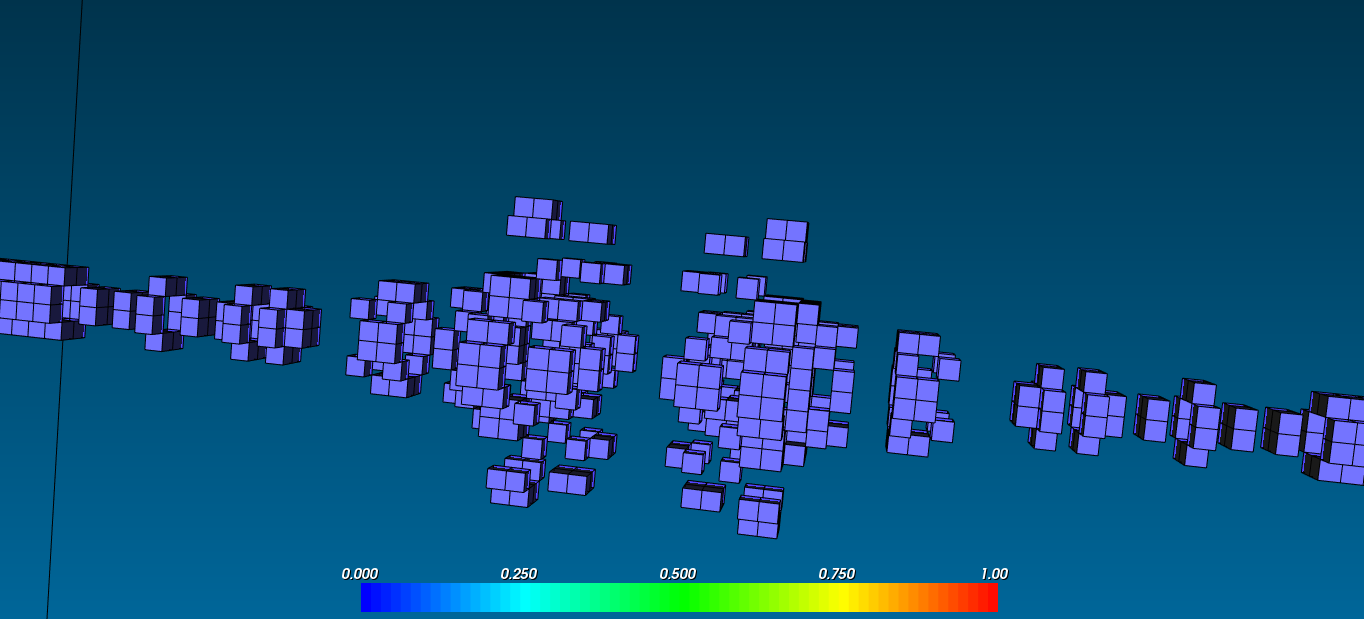
\includegraphics[scale=0.3]{pentominoes_ss/q_50_gliders.png}
	\caption{Evolution of the Q-Pentomino, zoomed gliders, $50^{th}$ generation.}
  \label{fig:ss-pent:q-50-gliders}
\end{figure}

\begin{figure}
	\centering
	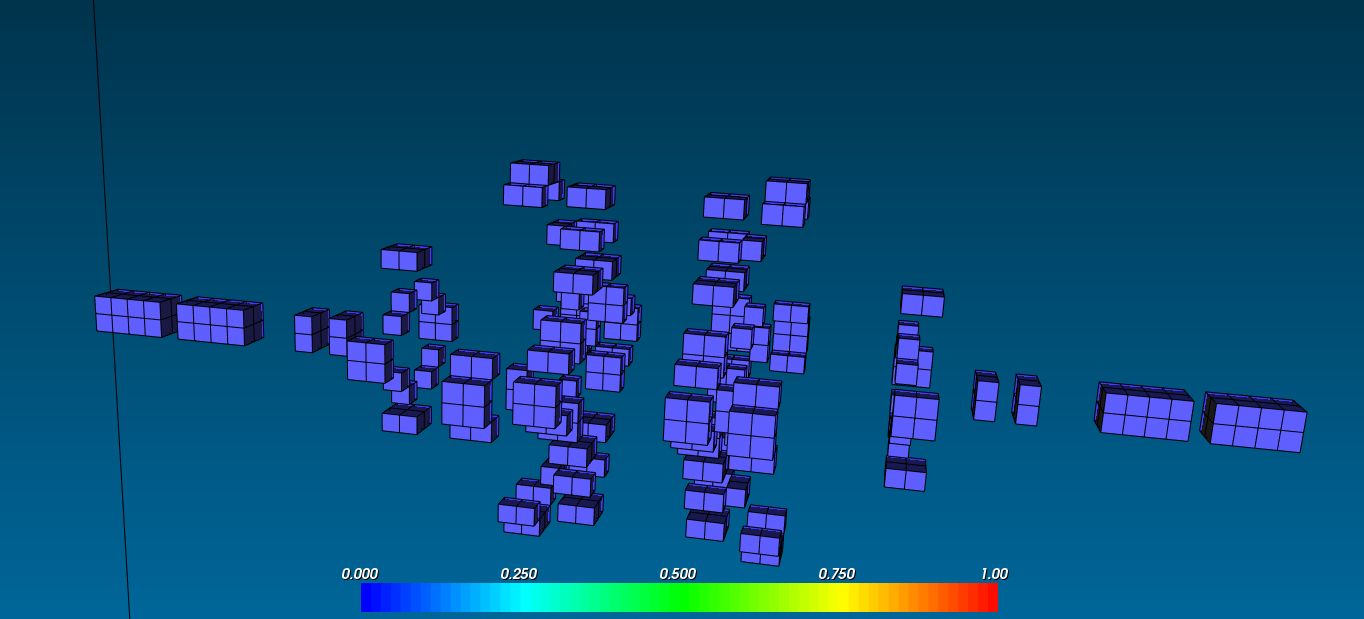
\includegraphics[scale=0.3]{pentominoes_ss/q_52_gliders.png}
	\caption{Evolution of the Q-Pentomino, zoomed gliders, $52^{th}$ generation.}
  \label{fig:ss-pent:q-52-gliders}
\end{figure}

% R PENTOMINO ==================================================================
\subsubsection{R-Pentomino}
\label{sec:r-pentomino}
This pentomino (see figure~\ref{fig:iso-pent-r}), just like it's equivalent in
two dimensions, expands very quickly in a short period of time, this can be seen
in the figure~\ref{fig:ss-pent:r-comparative}, where a comparative between the
evolution achieved in the same generation for different pentominos.

The puffer train (see figure~\ref{fig:iso-puffer-1}) appears here, too; as the
glider-1 (see figure~\ref{fig:iso-glider-1}) and glider-4 (see
figure~\ref{fig:iso-glider-4}); the gliders can be seen in the  $81^{th}$
generation, in the north-east, nort-west, south-east and south-west areas of the
figure~\ref{fig:ss-pent:r-81}; in the figure~\ref{fig:ss-pent:r-81-glider1}, a
pair of glider-1 can be seen easily in the left of the figure; the glider-4 is
shown in the upper-left of figure~\ref{fig:ss-pent:r-81-glider4}.

\begin{figure}
	\centering
	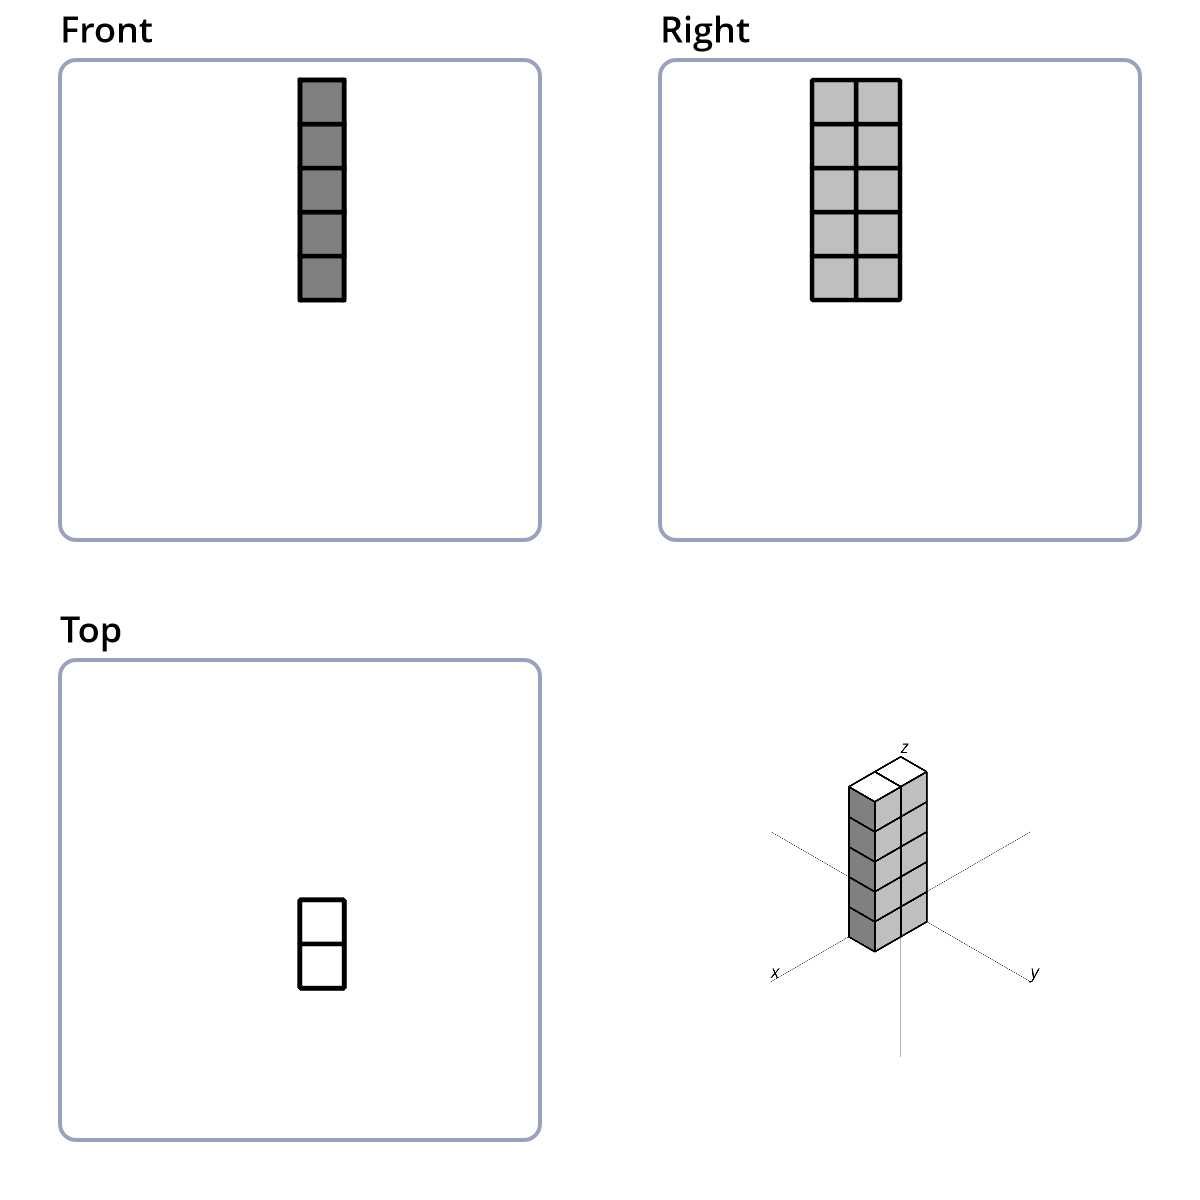
\includegraphics[scale=0.3]{iso_diagrams/o.png}
	\caption{Isometric of the R-pentomino.}
  \label{fig:iso-pent-r}
\end{figure}

\begin{figure}
	\centering
	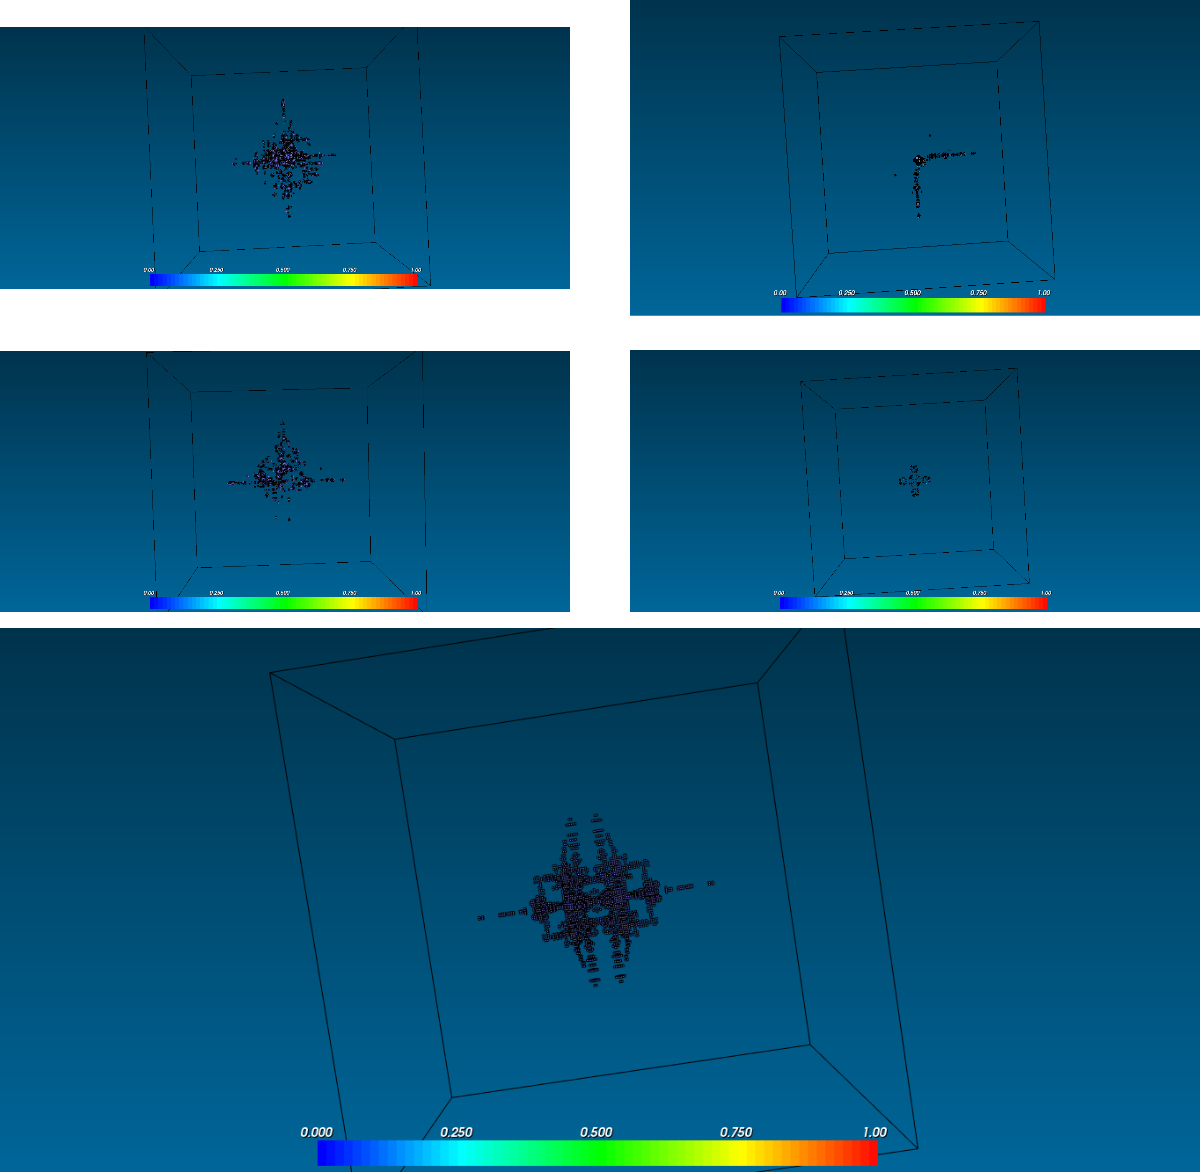
\includegraphics[scale=0.4]{pentominoes_ss/r-comparative-70g.png}
	\caption{Evolution in the $52^{th}$ generation for the Y, W, P, X and R
	pentominoes respectively.}
  \label{fig:ss-pent:r-comparative}
\end{figure}

\begin{figure}
	\centering
	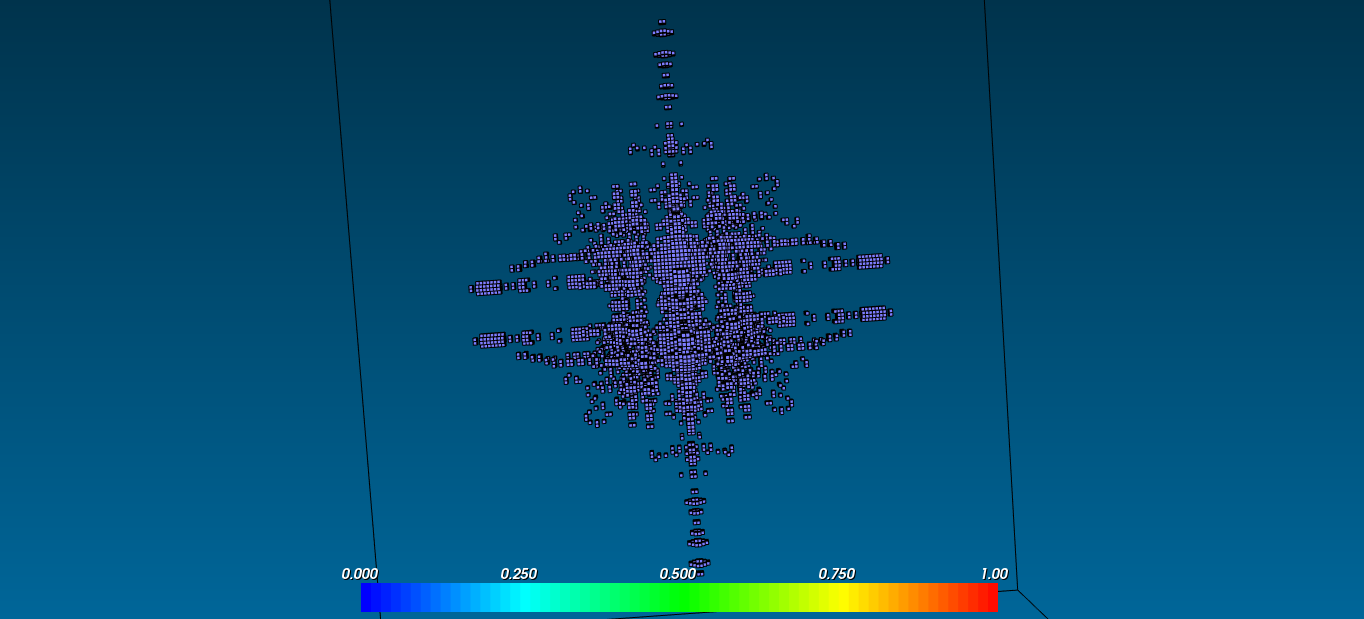
\includegraphics[scale=0.3]{pentominoes_ss/r_81.png}
	\caption{Evolution of the Q-Pentomino, $81^{th}$ generation.}
  \label{fig:ss-pent:r-81}
\end{figure}

\begin{figure}
	\centering
	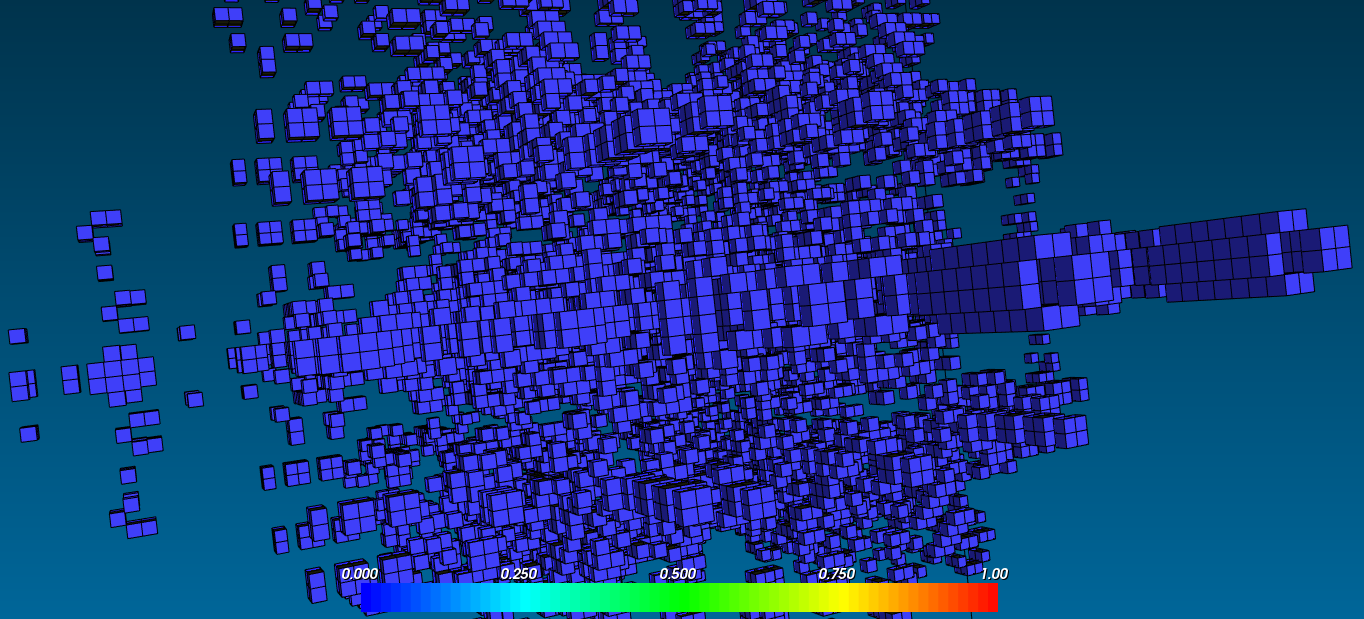
\includegraphics[scale=0.3]{pentominoes_ss/r_81_glider1.png}
	\caption{Evolution of the Q-Pentomino, zoomed glider-1, $81^{th}$ generation.}
  \label{fig:ss-pent:r-81-glider1}
\end{figure}

\begin{figure}
	\centering
	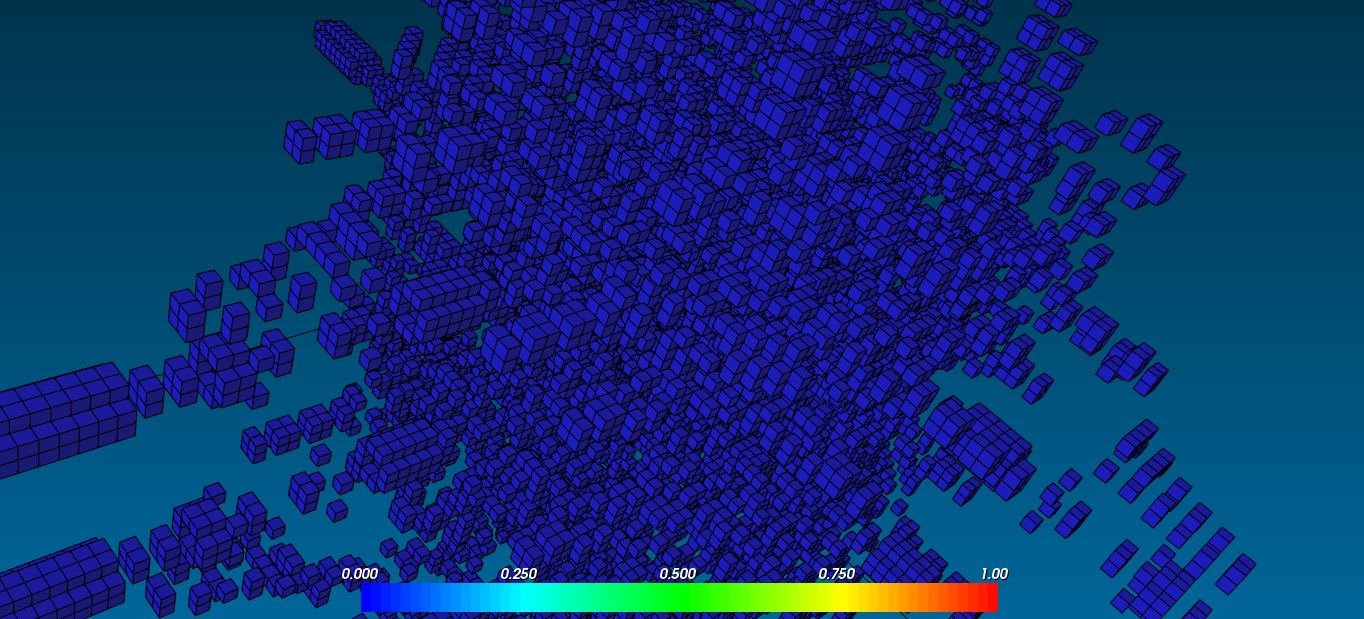
\includegraphics[scale=0.3]{pentominoes_ss/r_81_glider4.png}
	\caption{Evolution of the Q-Pentomino, zoomed glider-4, $81^{th}$ generation.}
  \label{fig:ss-pent:r-81-glider4}
\end{figure}

% S PENTOMINO ==================================================================
\subsubsection{S-Pentomino}
\label{sec:s-pentomino}
This pentomino (see figure~\ref{fig:iso-pent-s}),


\begin{figure}
	\centering
	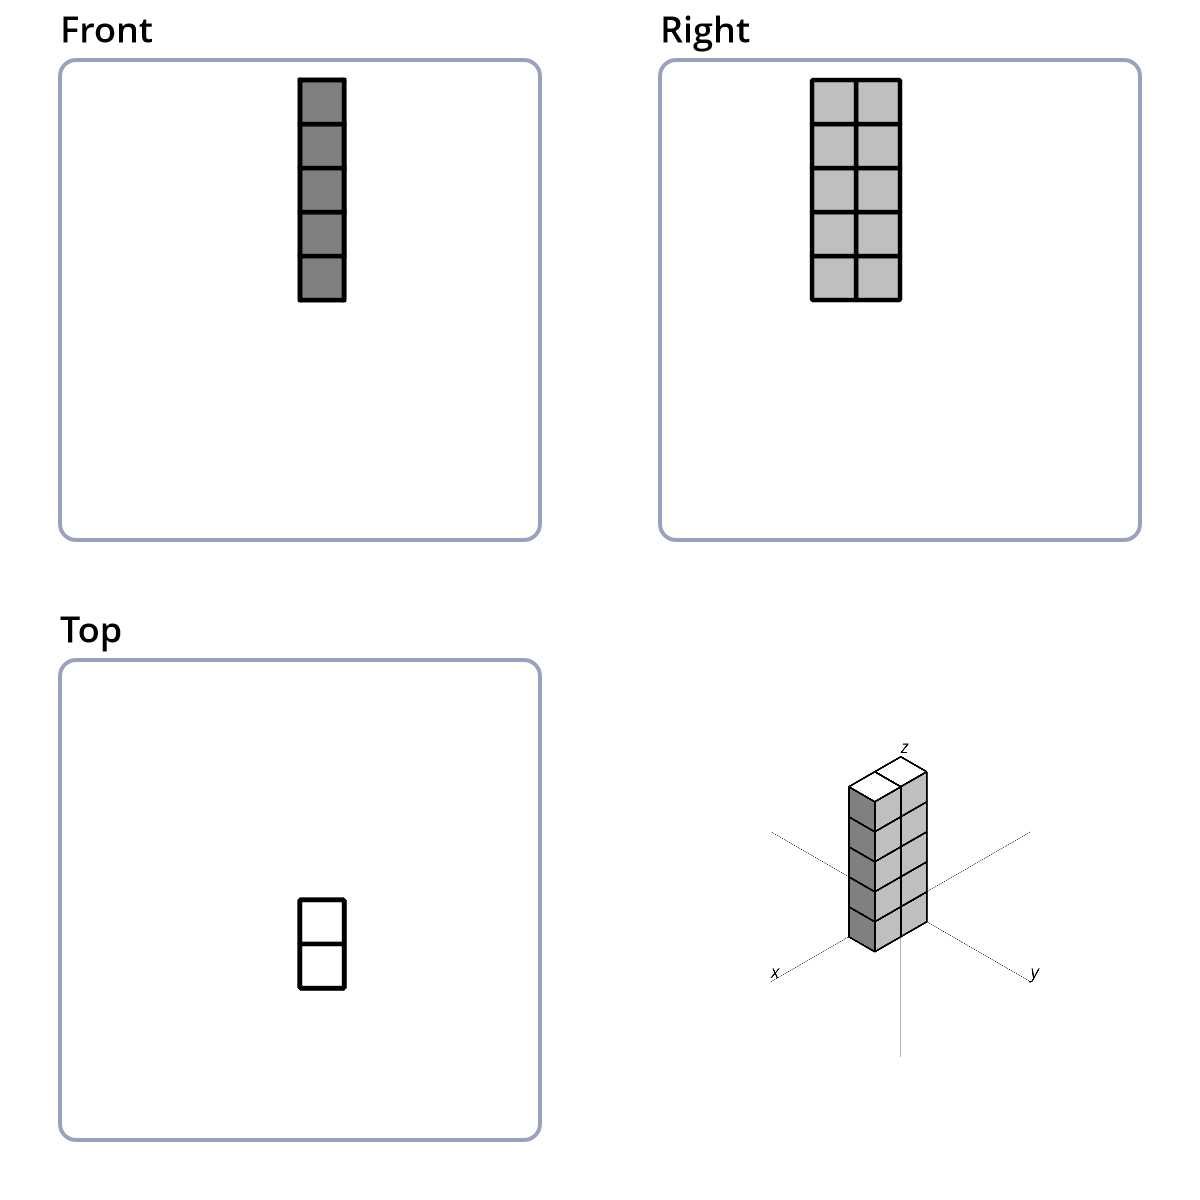
\includegraphics[scale=0.3]{iso_diagrams/o.png}
	\caption{Isometric of the S-pentomino.}
  \label{fig:iso-pent-s}
\end{figure}

% T PENTOMINO ==================================================================
\subsubsection{T-Pentomino}
\label{sec:t-pentomino}
This pentomino (see figure~\ref{fig:iso-pent-t}),


\begin{figure}
	\centering
	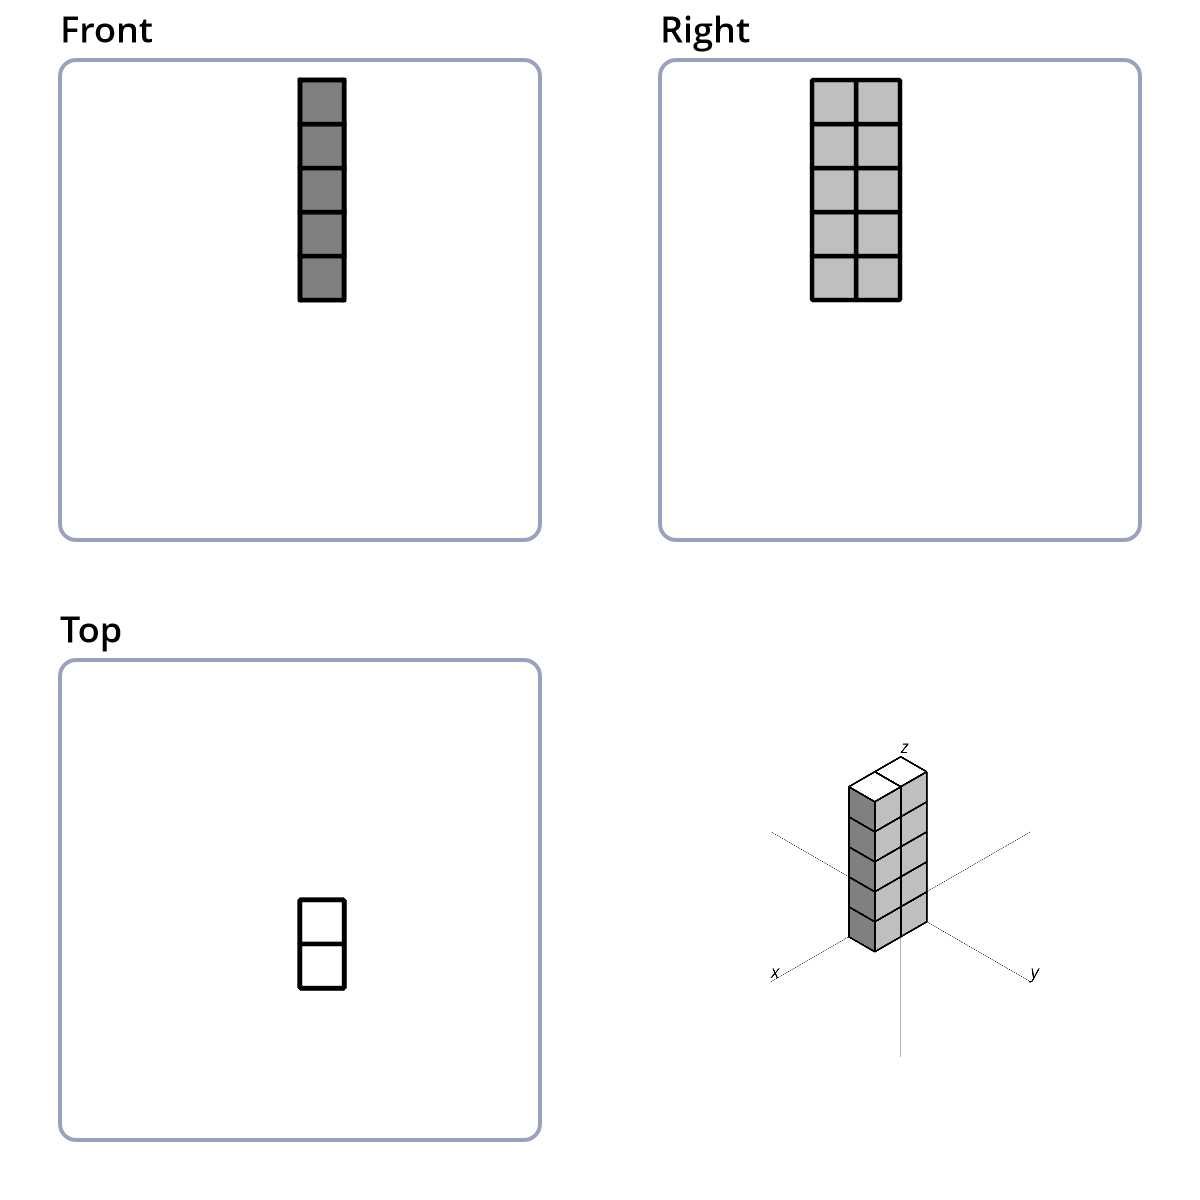
\includegraphics[scale=0.3]{iso_diagrams/o.png}
	\caption{Isometric of the T-pentomino.}
  \label{fig:iso-pent-t}
\end{figure}

\subsubsection{U-Pentomino}
\label{sec:u-pentomino}
This pentomino (see figure~\ref{fig:iso-pent-u}),


\begin{figure}
	\centering
	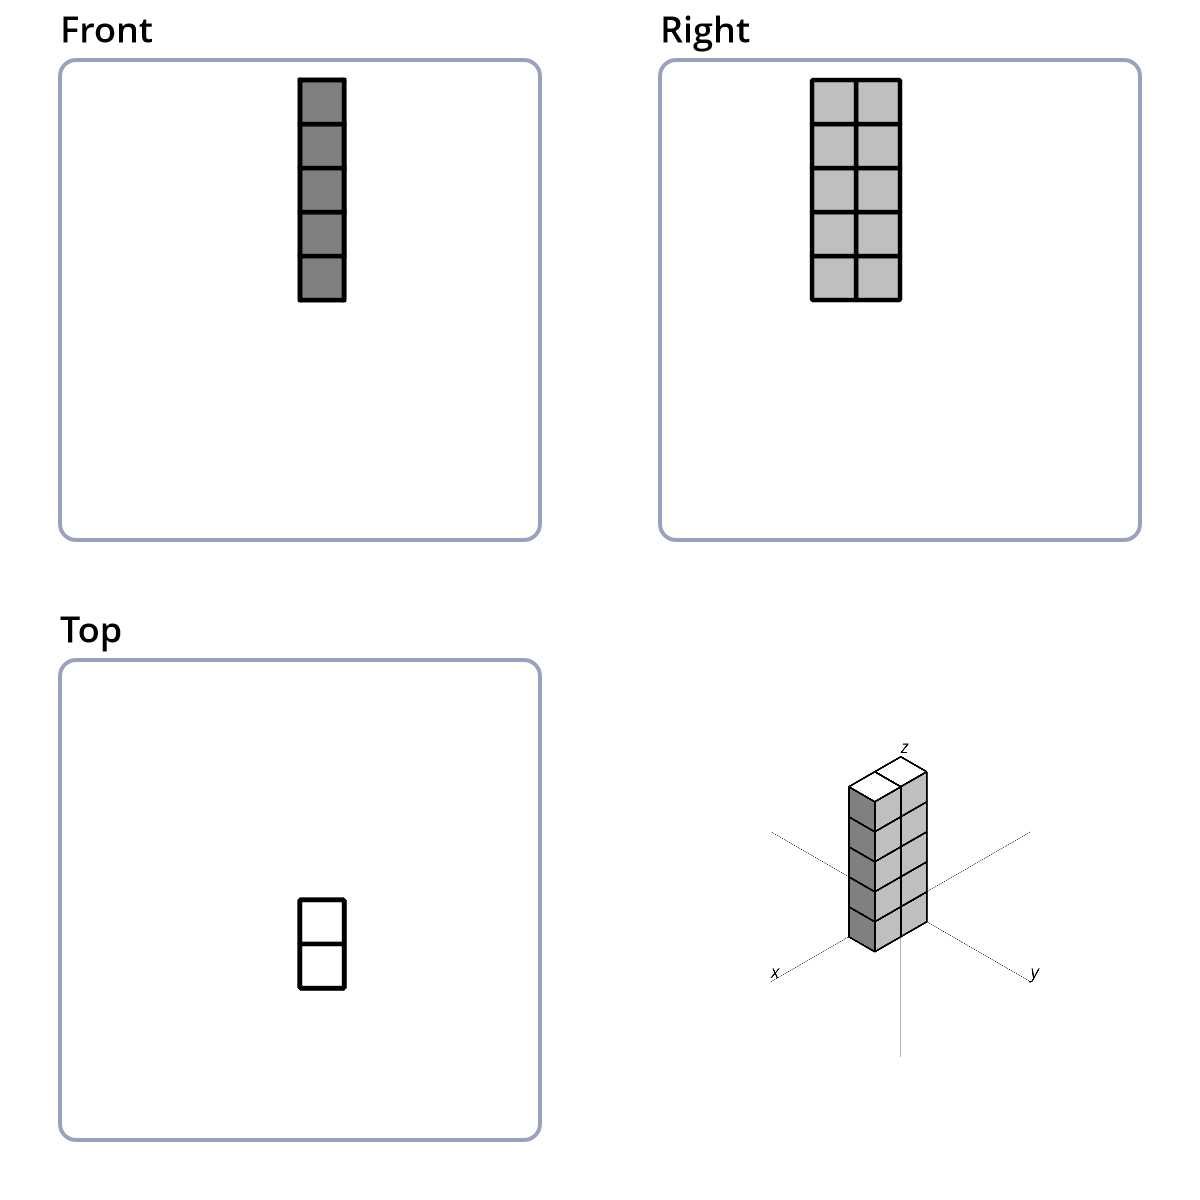
\includegraphics[scale=0.3]{iso_diagrams/o.png}
	\caption{Isometric of the U-pentomino.}
  \label{fig:iso-pent-u}
\end{figure}
\subsubsection{V-Pentomino}
\label{sec:v-pentomino}
This pentomino (see figure~\ref{fig:iso-pent-v}),


\begin{figure}
	\centering
	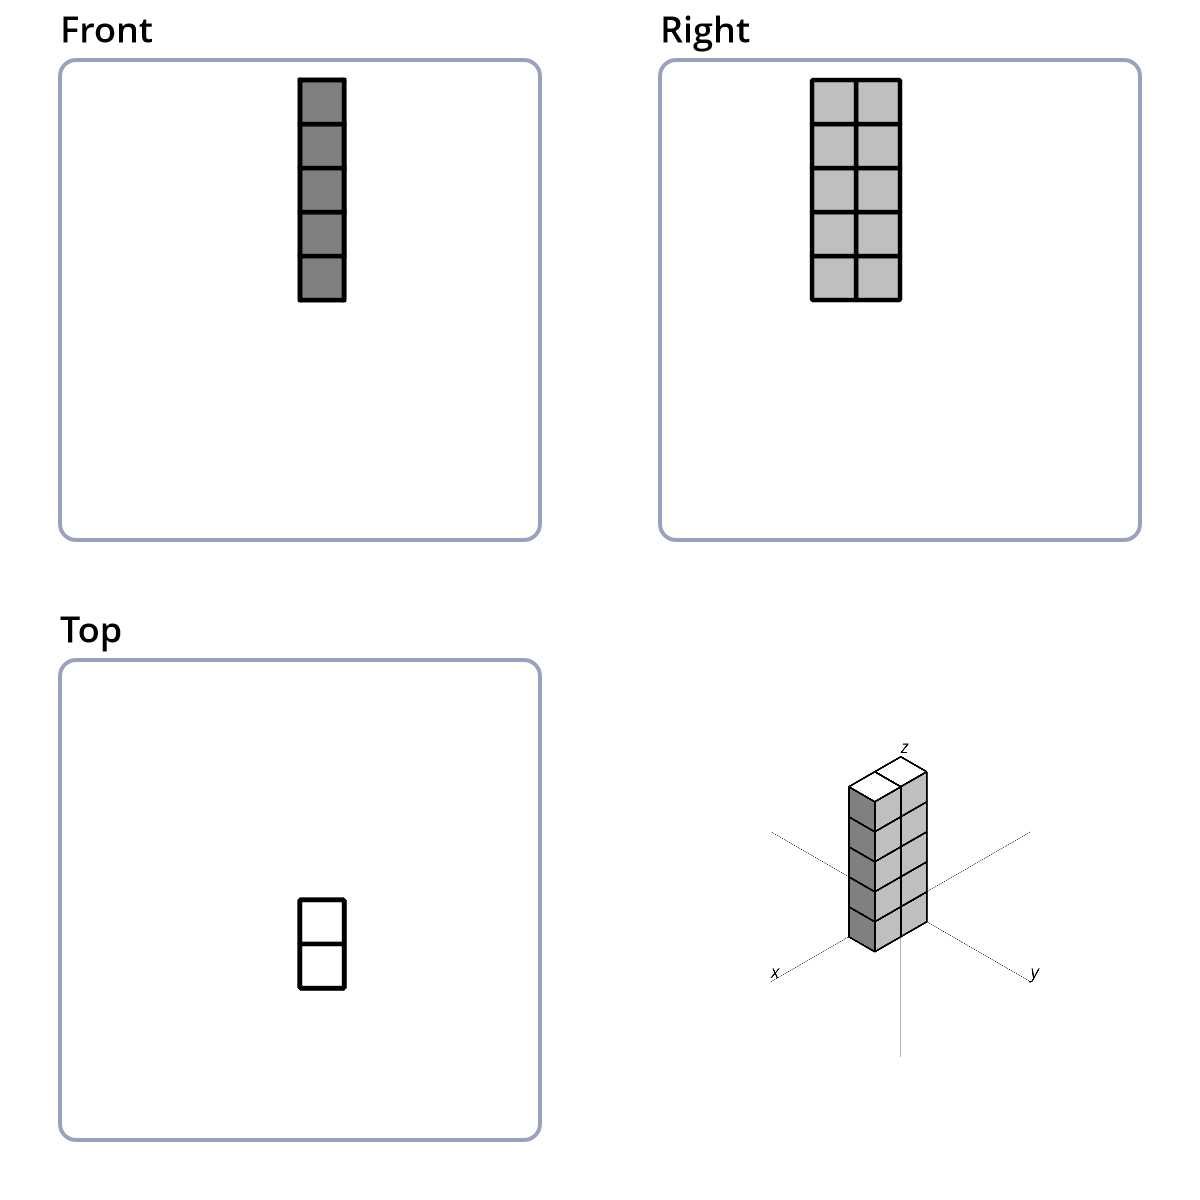
\includegraphics[scale=0.3]{iso_diagrams/o.png}
	\caption{Isometric of the V-pentomino.}
  \label{fig:iso-pent-v}
\end{figure}
\subsubsection{W-Pentomino}
\label{sec:w-pentomino}
This pentomino (see figure~\ref{fig:iso-pent-w}),


\begin{figure}
	\centering
	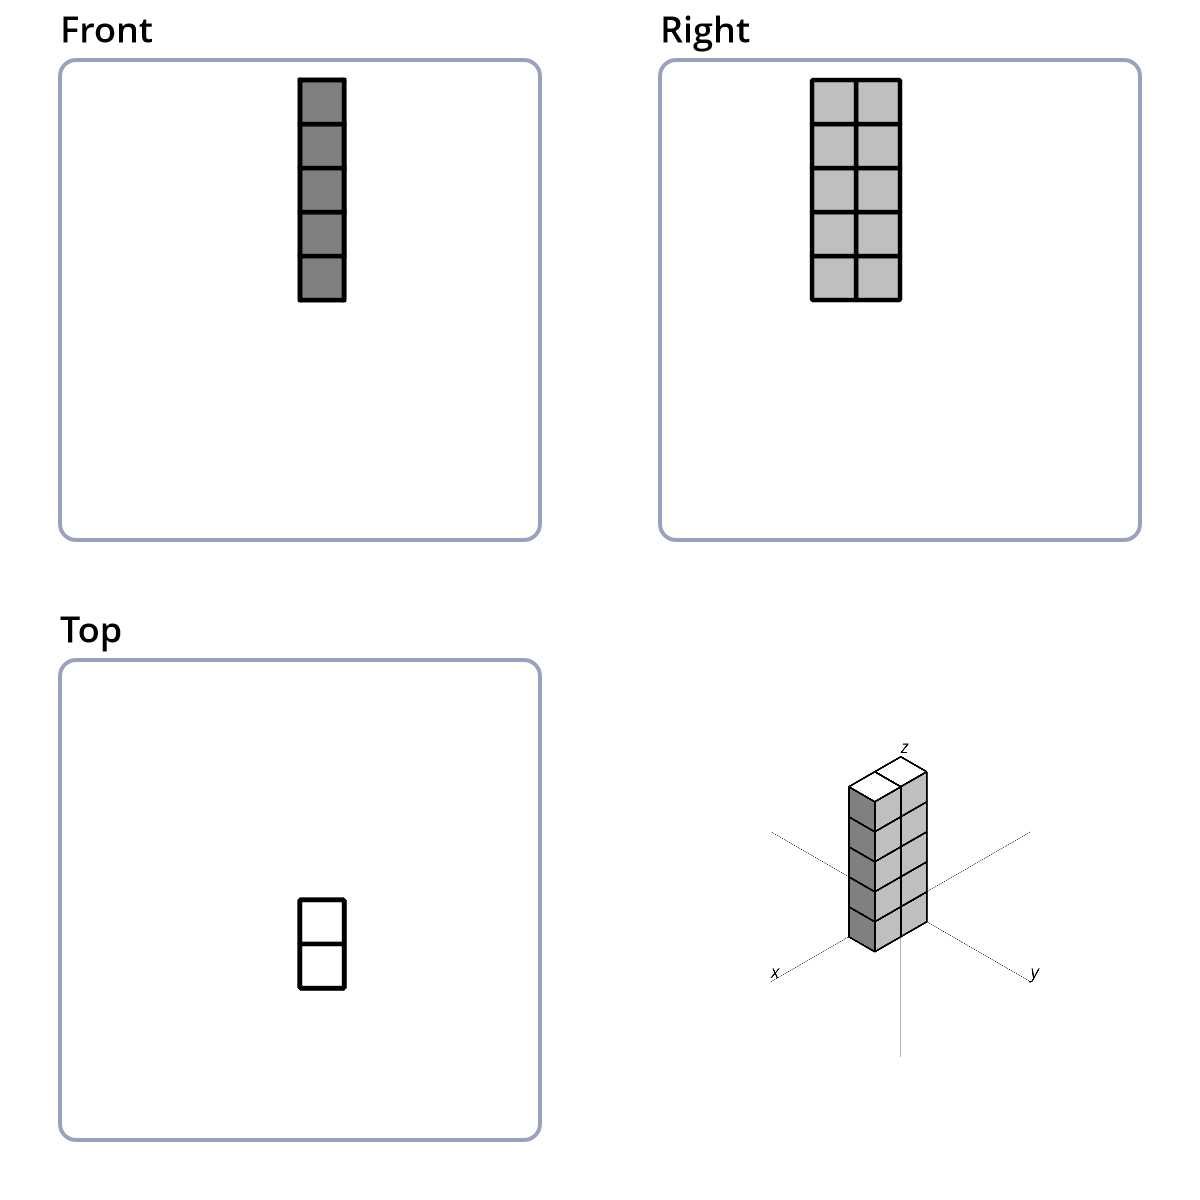
\includegraphics[scale=0.3]{iso_diagrams/o.png}
	\caption{Isometric of the W-pentomino.}
  \label{fig:iso-pent-w}
\end{figure}
\subsubsection{X-Pentomino}
\label{sec:x-pentomino}
This pentomino (see figure~\ref{fig:iso-pent-x}),


\begin{figure}
	\centering
	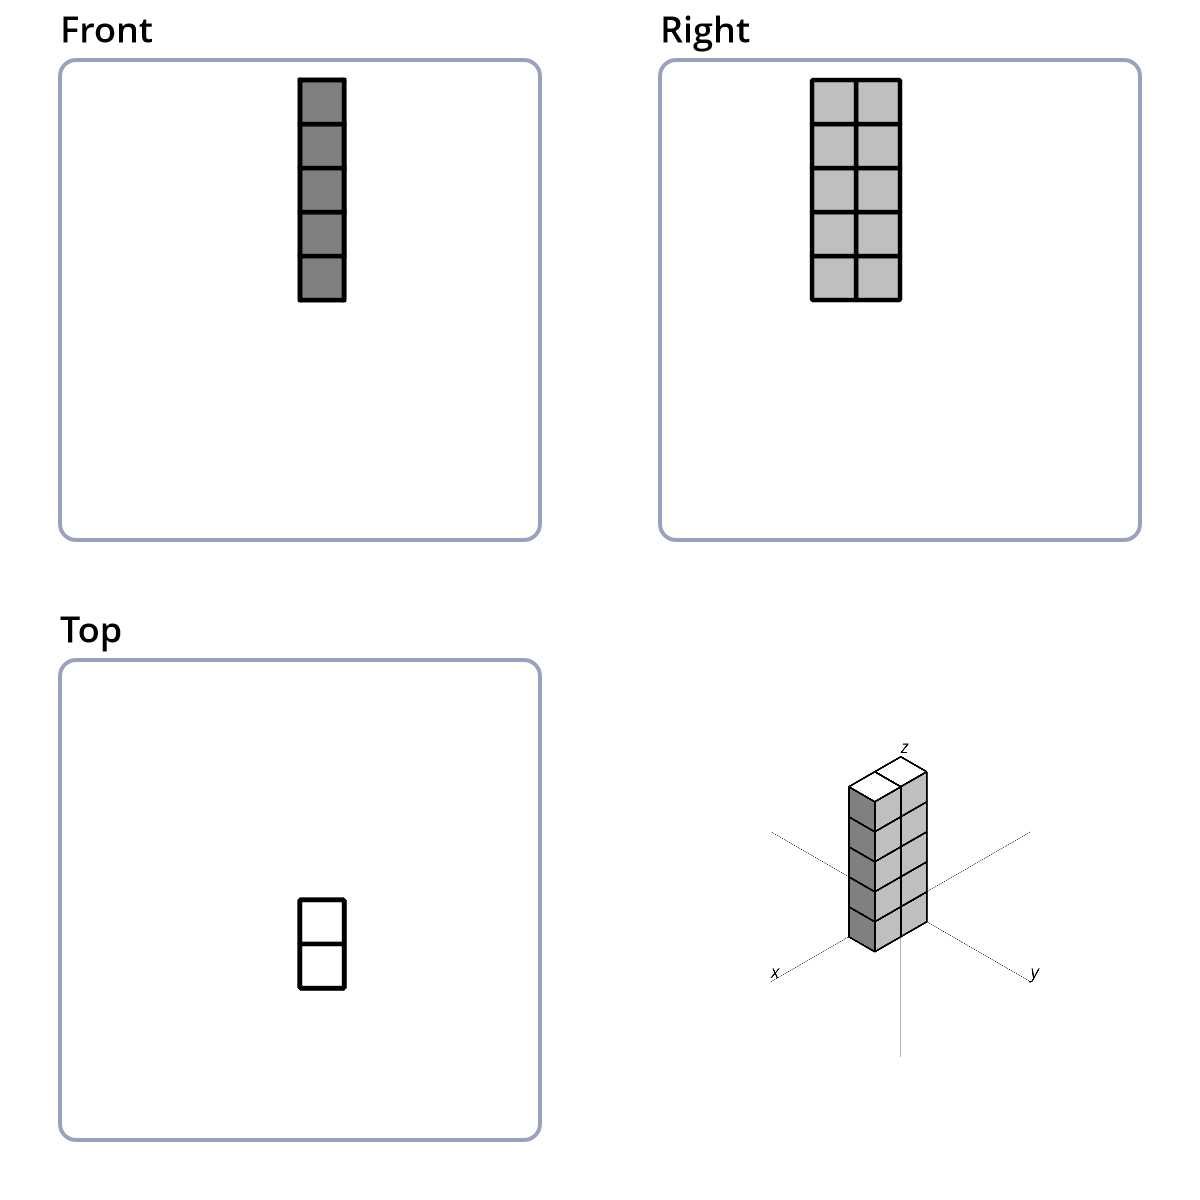
\includegraphics[scale=0.3]{iso_diagrams/o.png}
	\caption{Isometric of the X-pentomino.}
  \label{fig:iso-pent-x}
\end{figure}
\subsubsection{Y-Pentomino}
\label{sec:y-pentomino}
This pentomino (see figure~\ref{fig:iso-pent-y}),


\begin{figure}
	\centering
	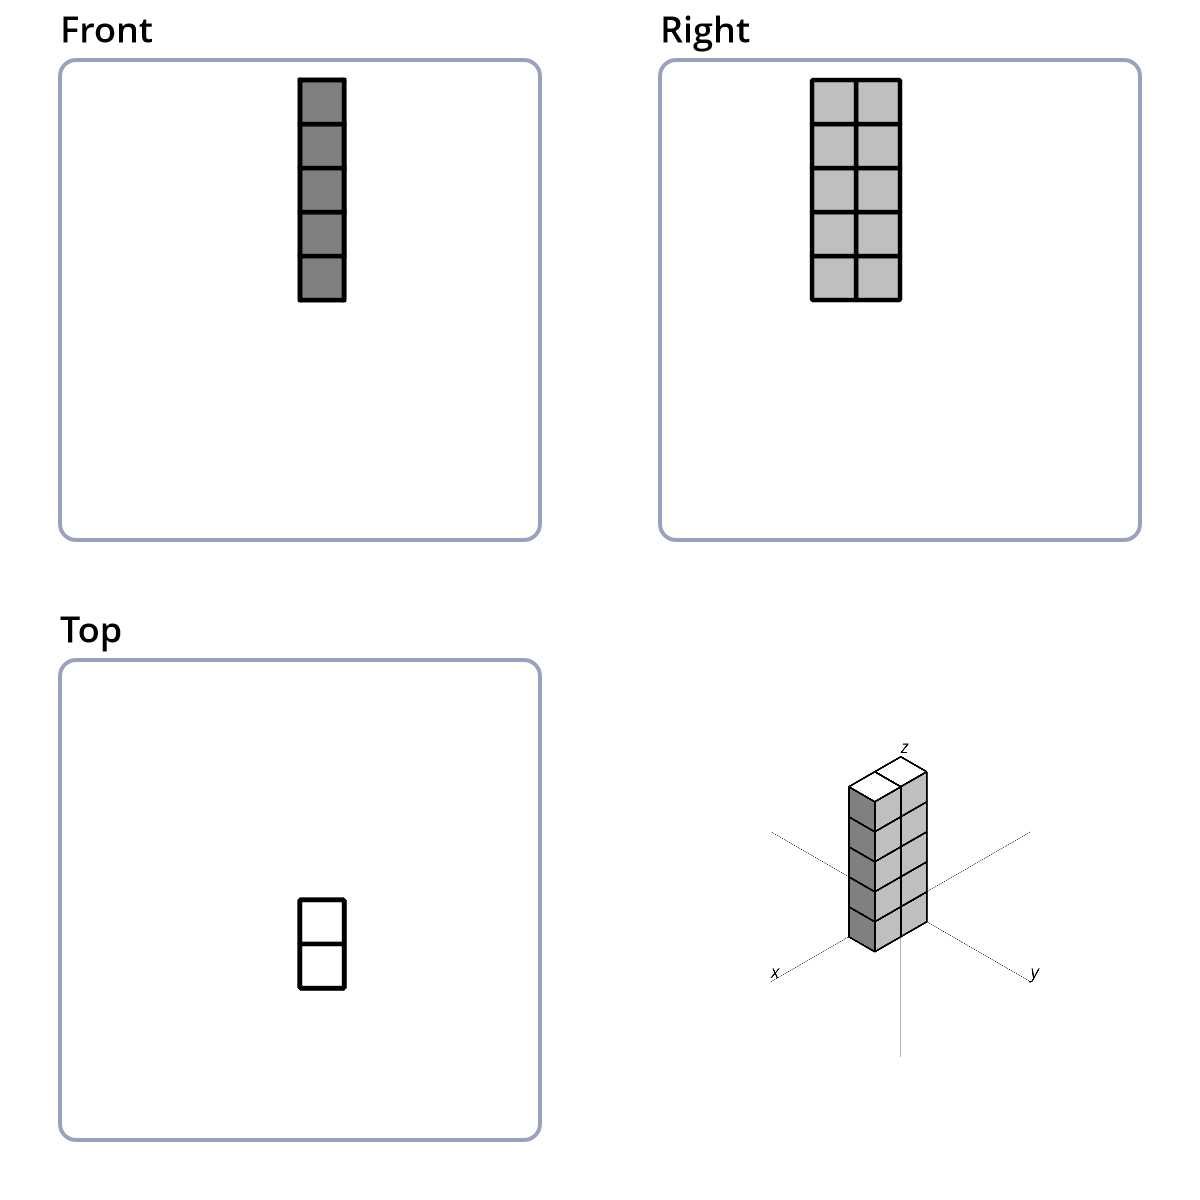
\includegraphics[scale=0.3]{iso_diagrams/o.png}
	\caption{Isometric of the Y-pentomino.}
  \label{fig:iso-pent-y}
\end{figure}
\subsubsection{Z-Pentomino}
\label{sec:z-pentomino}
This pentomino (see figure~\ref{fig:iso-pent-z}),


\begin{figure}
	\centering
	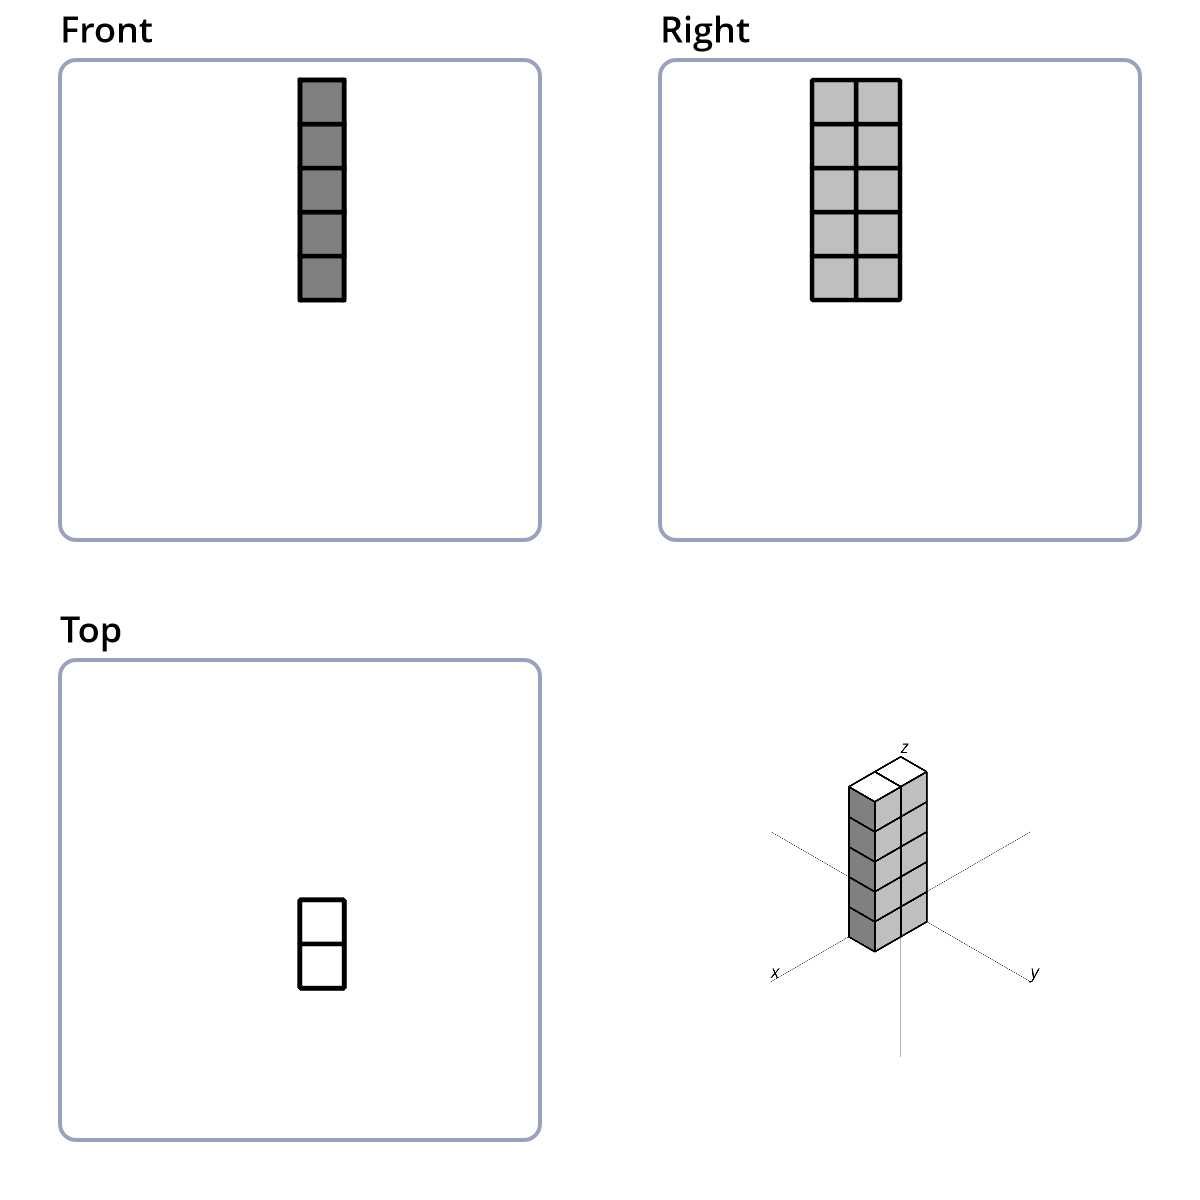
\includegraphics[scale=0.3]{iso_diagrams/o.png}
	\caption{Isometric of the Z-pentomino.}
  \label{fig:iso-pent-z}
\end{figure}
